
\documentclass[a4paper,11pt]{article}

\usepackage[utf8]{inputenc}
\usepackage[T1]{fontenc}
\usepackage[french]{babel}

\usepackage{geometry}
\geometry{margin=2.5cm}

\usepackage{graphicx}
\usepackage{listings}
\usepackage{xcolor}
\usepackage{hyperref}

\title{Robo Rescue\\Rapport Technique}
\author{Lionel DOFONHAKOU}
\date{\today}

\begin{document}

\maketitle

\tableofcontents

\newpage

\section{Introduction}

Robo Rescue est un jeu de type labyrinthe développé en langage C à l'aide de la bibliothèque SDL2.

Le joueur contrôle un robot qui doit atteindre une étoile représentant la sortie du niveau tout en gérant plusieurs ressources limitées.

L'objectif principal de ce projet n'était pas uniquement de produire un jeu fonctionnel mais également de se familiariser avec le développement graphique en C à l'aide de SDL2 et de consolider plusieurs notions fondamentales étudiées durant les enseignements de programmation.

Parmi les notions révisées figurent notamment :

\begin{itemize}
    \item la programmation modulaire ;
    \item les structures de données ;
    \item les énumérations ;
    \item les pointeurs ;
    \item l'allocation dynamique ;
    \item la gestion mémoire ;
    \item les Makefiles ;
    \item le débogage avec Valgrind.
\end{itemize}



\section{Aperçu du jeu}

La Figure~\ref{fig:gameplay} présente une capture d'écran de l'interface graphique du jeu.

\begin{figure}[h]
    \centering
    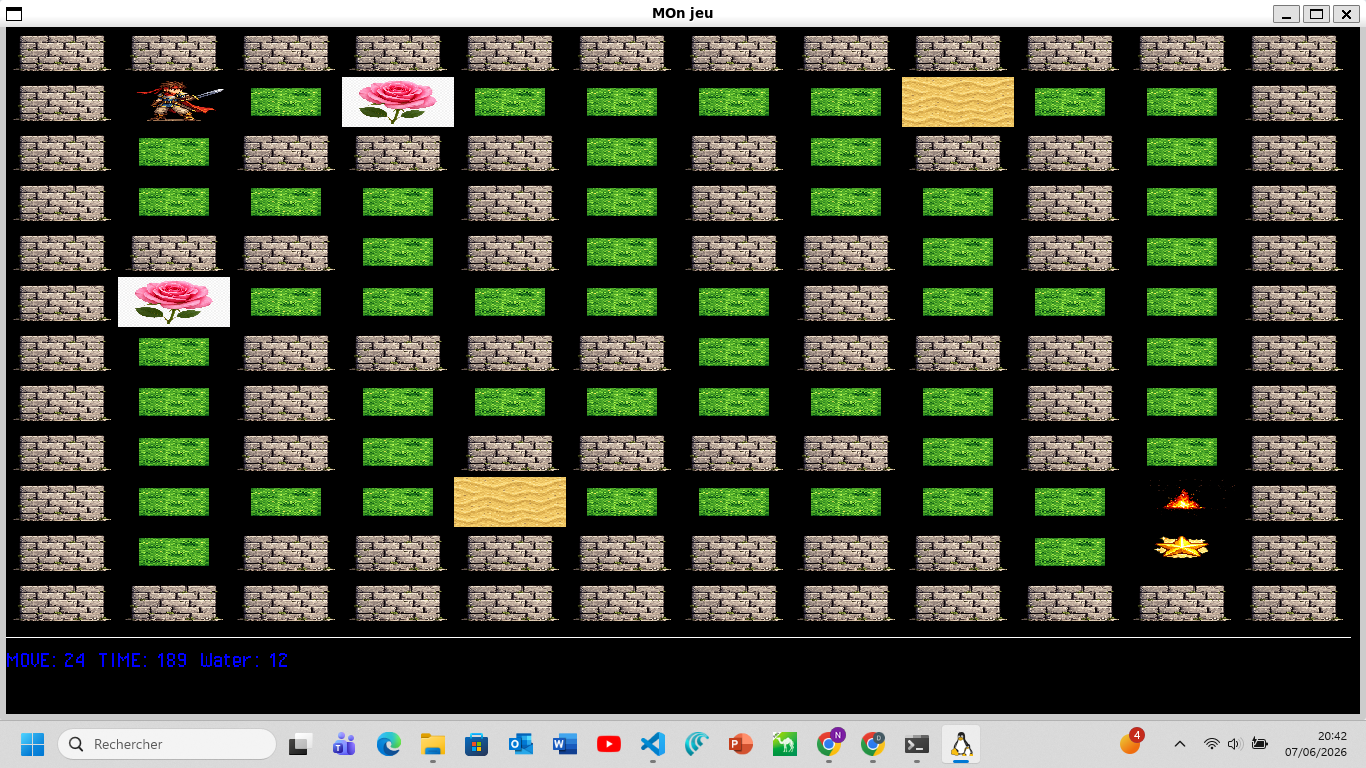
\includegraphics[width=0.9\textwidth]{../display/Capture d'écran 2026-06-07 204255.png}
    \caption{Capture d'écran de Robo Rescue}
    \label{fig:gameplay}
\end{figure}

L'interface est composée de plusieurs éléments :

\begin{itemize}
    \item la carte du niveau ;
    \item le joueur représenté par un robot ;
    \item les différents types de terrain ;
    \item l'étoile indiquant la sortie ;
    \item l'affichage des ressources du joueur ;
    \item les messages de victoire ou d'échec.
\end{itemize}


\section{Architecture générale du projet}

Le projet est organisé en plusieurs modules indépendants.

\begin{itemize}
    \item \texttt{map.c / map.h} : gestion des cartes.
    \item \texttt{player.c / player.h} : gestion du joueur.
    \item \texttt{game.c / game.h} : logique du jeu.
    \item \texttt{render.c / render.h} : affichage SDL.
    \item \texttt{main.c} : boucle principale.
\end{itemize}

Cette organisation permet de séparer les responsabilités et d'obtenir un code plus lisible et maintenable.

\section{Structures de données}

\subsection{Position}

Toutes les positions du jeu sont représentées par :

\begin{lstlisting}[language=C]
struct location_t {
    int x;
    int y;
};
\end{lstlisting}

Cette structure est utilisée pour :

\begin{itemize}
    \item la position du joueur ;
    \item la position de sortie ;
    \item les futurs objets mobiles.
\end{itemize}

\subsection{Carte}

La carte est stockée sous forme de matrice dynamique.

\begin{lstlisting}[language=C]
struct map_t {
    enum ground_t **grid;
    int width;
    int height;
};
\end{lstlisting}

Chaque case contient un type de terrain :

\begin{itemize}
    \item GRASS
    \item FLOWER
    \item FIRE
    \item SAND
    \item WALL
\end{itemize}

Le chargement est effectué à partir d'un fichier texte contenant les dimensions puis les valeurs de la grille.

\subsection{Joueur}

\begin{lstlisting}[language=C]
struct player_t {
    struct location_t player_pos;
    int resources[NB_RESOURCES];
};
\end{lstlisting}

Le joueur possède :

\begin{itemize}
    \item une position ;
    \item des points de déplacement ;
    \item une réserve d'eau ;
    \item un temps restant.
\end{itemize}

\subsection{Jeu}

\begin{lstlisting}[language=C]
struct game_t {
    struct map_t map;
    struct player_t *player;
    struct location_t exit_location;
    struct location_t start_location;
};
\end{lstlisting}

Cette structure représente l'état complet d'une partie.

Elle constitue le lien entre tous les autres composants du programme.

\section{Gestion graphique avec SDL}

\subsection{Principe général}

Pour construire une application SDL, il faut retenir trois objets fondamentaux :

\begin{enumerate}
    \item SDL\_Window
    \item SDL\_Renderer
    \item SDL\_Texture
\end{enumerate}

La compréhension de ces trois concepts suffit à reconstruire la majorité des projets SDL.

\subsection{SDL\_Window}

Une fenêtre représente la zone visible de l'application.

Création :

\begin{lstlisting}[language=C]
SDL_CreateWindow(...)
\end{lstlisting}

Rôle :

\begin{itemize}
    \item définir la taille de la fenêtre ;
    \item définir son titre ;
    \item permettre le redimensionnement.
\end{itemize}

\subsection{SDL\_Renderer}

Le renderer est l'objet le plus important de SDL.

On peut le voir comme le moteur de dessin de l'application.

Toutes les opérations graphiques transitent par lui.

Création :

\begin{lstlisting}[language=C]
SDL_CreateRenderer(...)
\end{lstlisting}

Fonctions principales :

\begin{itemize}
    \item effacer l'écran ;
    \item dessiner des images ;
    \item dessiner des lignes ;
    \item dessiner des rectangles ;
    \item afficher le résultat final.
\end{itemize}

\subsection{SDL\_Texture}

Une texture correspond à une image stockée en mémoire graphique.

Dans le projet :

\begin{itemize}
    \item player.png
    \item grass.png
    \item wall.png
    \item flower.png
    \item fire.png
    \item sand.png
    \item star.png
\end{itemize}

sont converties en textures grâce à :

\begin{lstlisting}[language=C]
IMG_Load(...)
SDL_CreateTextureFromSurface(...)
\end{lstlisting}

\section{Cycle de rendu SDL}

Chaque image affichée à l'écran suit le même cycle.

\subsection{Étape 1 : Effacer l'écran}

\begin{lstlisting}[language=C]
SDL_RenderClear(renderer);
\end{lstlisting}

Permet de supprimer l'image précédente.

\subsection{Étape 2 : Dessiner les éléments}

Toutes les textures sont dessinées avec :

\begin{lstlisting}[language=C]
SDL_RenderCopy(...)
\end{lstlisting}

Cette fonction est probablement la plus utilisée dans tout projet SDL.

\subsection{Étape 3 : Afficher le résultat}

\begin{lstlisting}[language=C]
SDL_RenderPresent(renderer);
\end{lstlisting}

Le contenu du renderer devient visible.

\section{Gestion des événements}

SDL utilise une file d'événements.

La récupération des événements se fait grâce à :

\begin{lstlisting}[language=C]
SDL_PollEvent(...)
\end{lstlisting}

Dans Robo Rescue, les événements utilisés sont :

\begin{itemize}
    \item flèche haut ;
    \item flèche bas ;
    \item flèche gauche ;
    \item flèche droite ;
    \item fermeture de la fenêtre.
\end{itemize}

\section{Affichage de texte}

SDL ne gère pas directement les polices.

L'extension SDL\_ttf est nécessaire.

Étapes :

\begin{enumerate}
    \item Charger la police.
    \item Générer une surface texte.
    \item Transformer la surface en texture.
    \item Afficher la texture.
\end{enumerate}

Fonctions à retenir :

\begin{lstlisting}[language=C]
TTF_OpenFont(...)
TTF_RenderText_Solid(...)
SDL_CreateTextureFromSurface(...)
SDL_RenderCopy(...)
\end{lstlisting}

\section{Musique et effets sonores}

SDL\_mixer permet de gérer l'audio.

Fonctions importantes :

\begin{lstlisting}[language=C]
Mix_OpenAudio(...)
Mix_LoadMUS(...)
Mix_PlayMusic(...)
Mix_FreeMusic(...)
\end{lstlisting}

Ces fonctions permettent d'ajouter une musique de fond ainsi que des effets sonores.

\section{Mémo SDL pour les futurs projets}

Si je devais recommencer un projet SDL dans plusieurs années, la procédure à suivre serait :

\begin{enumerate}
    \item Initialiser SDL avec SDL\_Init().
    \item Créer une fenêtre avec SDL\_CreateWindow().
    \item Créer un renderer avec SDL\_CreateRenderer().
    \item Charger les textures avec SDL\_image.
    \item Mettre en place une boucle principale.
    \item Récupérer les événements avec SDL\_PollEvent().
    \item Dessiner les textures avec SDL\_RenderCopy().
    \item Afficher le résultat avec SDL\_RenderPresent().
    \item Libérer toutes les ressources à la fermeture.
\end{enumerate}

Cette séquence constitue le squelette de quasiment toutes les applications SDL2.

\section{Conclusion}

Ce projet a permis de découvrir concrètement le développement graphique en langage C avec SDL2.

Au-delà de l'aspect ludique, il a servi de support pour réviser de nombreuses notions fondamentales de programmation tout en développant une meilleure compréhension de l'organisation d'un projet logiciel complet.

Les connaissances acquises durant ce projet constituent une base solide pour le développement de futures applications graphiques ou de jeux vidéo plus complexes.

\end{document}
